% =====================================================================
% §2 Threat Landscape & Adversary Behaviour 
% =====================================================================

\section{Threat Landscape and Adversary Behaviour}
\label{sec:threat_landscape}

This section approaches adversary behaviour from three perspectives. First, two conceptual lenses: MITRE ATT\&CK (Section~\ref{subsec:mitre}), which gives that behaviour a shared, technique-level vocabulary, and the Pyramid of Pain (Section~\ref{subsec:pop}), which ranks indicator classes by the cost their disruption imposes on the adversary. Second, the adversary: the advanced persistent threat (Section~\ref{subsec:apt}), whose tradecraft is documented and durable enough to make behavioural modelling both tractable and worthwhile. Third, the method: attack profiling (Section~\ref{subsec:cti_profiling}), which reconstructs behaviour from raw cyber threat intelligence into structured, TTP-level representations.



\subsection{MITRE ATT\&CK}
\label{subsec:mitre}

The MITRE ATT\&CK framework is a knowledge base of adversary behaviours derived from real-world observations, developed by MITRE Corporation following its 2013 Fort Meade Experiment \cite{alsada2024}. ATT\&CK organises behaviour into a four-level hierarchy of tactics, techniques and sub-techniques, and procedures. A tactic refers to \textit{what} an attacker does to achieve a goal; a technique refers to \textit{how} that tactic is realised; a sub-technique refines a technique into a specific variant; a procedure is a particular instance of a technique, capturing the steps by which it has been implemented \cite{rodriguez2024}. The Initial Access tactic (TA0001), for example, may be realised through Phishing (T1566), via the Spearphishing Attachment sub-technique (T1566.001), with a procedure describing a crafted Office document whose macro executes a PowerShell payload on open.

ATT\&CK maintains three matrices --- Enterprise (IT networks and enterprise cloud), Mobile, and Industrial Control Systems --- of which Enterprise is the most heavily populated~\cite{alsada2024}.

Beyond the matrix itself, ATT\&CK catalogues named adversary groups (e.g., \texttt{G0016} for APT29), software (e.g., \texttt{S0154} for Cobalt Strike), and campaigns (e.g., \texttt{C0024} for the SolarWinds Compromise), each group characterised by the techniques observed across its operations~\cite{alsada2024}. These catalogues are serialised in Structured Threat Information Expression (STIX)~2.1, the standard machine-readable interchange format for CTI; among public STIX exports, the Enterprise bundle preserves the richest campaign-level structure~\cite{ferraz2026}, which is why this review centres on it. ATT\&CK has become the \emph{lingua franca} for adversary behaviour~\cite{buchel2025, ferraz2026}. Its distinguishing contribution is technique-level granularity --- finer than the phase-level Cyber Kill Chain or category-level STRIDE~\cite{alsada2024}.

Yet this serialisation --- the ATT\&CK-in-STIX export --- records \emph{which} techniques an adversary used without recording \emph{how} they fit together: it encodes no temporal order, explicit prerequisites, environmental constraints, or branching logic between techniques~\cite{ferraz2026}. Attack Flow, a STIX~2.1 extension language released by MITRE Engenuity's Center for Threat-Informed Defense (CTID) in 2022, supplies exactly this missing structure, representing the sequence and dependency relationships between techniques observed in real incidents~\cite{ctid2025attackflow}.

In a flow, actions (the ATT\&CK techniques) are joined by \emph{effect} edges that carry precondition semantics --- a downstream action cannot execute until the upstream one completes --- with AND/OR operators expressing multi-input dependencies and conditions capturing environmental state~\cite{ctid2025attackflow}. This is the structure a linear kill chain or flat intrusion-set membership cannot express: Figure~\ref{fig:attck-attackflow} reconstructs the 2018 Tesla cryptojacking incident on the model, where a three-input AND operator joins Deploy Container (T1610), Proxy (T1090), and Non-Standard Port (T1571) into Resource Hijacking (T1496).

CTID maintains a corpus of flows reconstructed by analysts from publicly reported incidents~\cite{ctid2025attackflow}. It is this analyst-curated corpus --- reliable structured behaviour bought at a coverage cost taken up in Section~\ref{subsec:cti_profiling} --- that supplies the data substrate for the adversarial profiles this review motivates.

\begin{figure*}[!t]
  \centering
  % =====================================================================
% Figure for lit-review §2.1 — Attack Flow excerpt (Tesla Kubernetes
% cryptojacking, 2018).
%
% Adapted from MITRE/CTID Attack Flow example corpus
% (`Tesla_Kubernetes_Breach.afb`). The figure carries §2.1 P3's claim
% that Attack Flow encodes precondition logic, sequencing, and
% dependency structure between MITRE ATT&CK techniques — i.e. it does
% what intrusion-set membership cannot.
%
% Pedagogical features visible in this excerpt:
%   (1) Condition object (green) — an environmental precondition (the
%       publicly-exposed Kubernetes dashboard) that gates the
%       initial-access action; only the `true' branch is realised.
%   (2) Fan-out from T1133 — two parallel attack paths (credential
%       exfiltration; cryptomining), demonstrating Attack Flow's
%       multi-path representation.
%   (3) AND operator (red) — three-input join in the cryptomining
%       branch; T1496 Resource Hijacking required deploy-container,
%       proxy, and non-standard-port all to succeed. The structural
%       feature a linear kill-chain or intrusion-set cannot express.
%   (4) Infrastructure object (grey cylinder) — a STIX-typed entity
%       (Unlisted mining pool) related to both T1583.004 and T1496
%       via `related-to' edges, illustrating that Attack Flow nodes
%       carry STIX objects beyond techniques themselves. Cylinder
%       shape signals that this is a different kind of node from
%       the action rectangles.
%   (5) Dagger marker (T1552) — the credential-branch path is analyst
%       speculation in the source, not observed activity; the figure
%       preserves provenance fidelity rather than presenting it as
%       fact. Explained in the in-figure legend.
%
% Edge conventions:
%   - Solid arrow (->): `effect' edge — downstream technique cannot
%     execute until upstream completes (Attack Flow's precondition
%     semantics).
%   - Dashed line (no head): `related-to' STIX relationship — no
%     causal ordering implied. Routed along outer columns (x=3.4 and
%     x=13.6), descending below the action grid and turning into
%     Infrastructure's west/east anchors, so neither dashed line
%     crosses any node.
%
% Required packages (loaded in main.tex preamble):
%   \usepackage{tikz}
%   \usetikzlibrary{positioning, arrows.meta, calc, shapes.geometric}
%   \usepackage{xcolor}
% Note: shapes.geometric is required for the cylinder infra style.
%
% Usage:
%   % =====================================================================
% Figure for lit-review §2.1 — Attack Flow excerpt (Tesla Kubernetes
% cryptojacking, 2018).
%
% Adapted from MITRE/CTID Attack Flow example corpus
% (`Tesla_Kubernetes_Breach.afb`). The figure carries §2.1 P3's claim
% that Attack Flow encodes precondition logic, sequencing, and
% dependency structure between MITRE ATT&CK techniques — i.e. it does
% what intrusion-set membership cannot.
%
% Pedagogical features visible in this excerpt:
%   (1) Condition object (green) — an environmental precondition (the
%       publicly-exposed Kubernetes dashboard) that gates the
%       initial-access action; only the `true' branch is realised.
%   (2) Fan-out from T1133 — two parallel attack paths (credential
%       exfiltration; cryptomining), demonstrating Attack Flow's
%       multi-path representation.
%   (3) AND operator (red) — three-input join in the cryptomining
%       branch; T1496 Resource Hijacking required deploy-container,
%       proxy, and non-standard-port all to succeed. The structural
%       feature a linear kill-chain or intrusion-set cannot express.
%   (4) Infrastructure object (grey cylinder) — a STIX-typed entity
%       (Unlisted mining pool) related to both T1583.004 and T1496
%       via `related-to' edges, illustrating that Attack Flow nodes
%       carry STIX objects beyond techniques themselves. Cylinder
%       shape signals that this is a different kind of node from
%       the action rectangles.
%   (5) Dagger marker (T1552) — the credential-branch path is analyst
%       speculation in the source, not observed activity; the figure
%       preserves provenance fidelity rather than presenting it as
%       fact. Explained in the in-figure legend.
%
% Edge conventions:
%   - Solid arrow (->): `effect' edge — downstream technique cannot
%     execute until upstream completes (Attack Flow's precondition
%     semantics).
%   - Dashed line (no head): `related-to' STIX relationship — no
%     causal ordering implied. Routed along outer columns (x=3.4 and
%     x=13.6), descending below the action grid and turning into
%     Infrastructure's west/east anchors, so neither dashed line
%     crosses any node.
%
% Required packages (loaded in main.tex preamble):
%   \usepackage{tikz}
%   \usetikzlibrary{positioning, arrows.meta, calc, shapes.geometric}
%   \usepackage{xcolor}
% Note: shapes.geometric is required for the cylinder infra style.
%
% Usage:
%   % =====================================================================
% Figure for lit-review §2.1 — Attack Flow excerpt (Tesla Kubernetes
% cryptojacking, 2018).
%
% Adapted from MITRE/CTID Attack Flow example corpus
% (`Tesla_Kubernetes_Breach.afb`). The figure carries §2.1 P3's claim
% that Attack Flow encodes precondition logic, sequencing, and
% dependency structure between MITRE ATT&CK techniques — i.e. it does
% what intrusion-set membership cannot.
%
% Pedagogical features visible in this excerpt:
%   (1) Condition object (green) — an environmental precondition (the
%       publicly-exposed Kubernetes dashboard) that gates the
%       initial-access action; only the `true' branch is realised.
%   (2) Fan-out from T1133 — two parallel attack paths (credential
%       exfiltration; cryptomining), demonstrating Attack Flow's
%       multi-path representation.
%   (3) AND operator (red) — three-input join in the cryptomining
%       branch; T1496 Resource Hijacking required deploy-container,
%       proxy, and non-standard-port all to succeed. The structural
%       feature a linear kill-chain or intrusion-set cannot express.
%   (4) Infrastructure object (grey cylinder) — a STIX-typed entity
%       (Unlisted mining pool) related to both T1583.004 and T1496
%       via `related-to' edges, illustrating that Attack Flow nodes
%       carry STIX objects beyond techniques themselves. Cylinder
%       shape signals that this is a different kind of node from
%       the action rectangles.
%   (5) Dagger marker (T1552) — the credential-branch path is analyst
%       speculation in the source, not observed activity; the figure
%       preserves provenance fidelity rather than presenting it as
%       fact. Explained in the in-figure legend.
%
% Edge conventions:
%   - Solid arrow (->): `effect' edge — downstream technique cannot
%     execute until upstream completes (Attack Flow's precondition
%     semantics).
%   - Dashed line (no head): `related-to' STIX relationship — no
%     causal ordering implied. Routed along outer columns (x=3.4 and
%     x=13.6), descending below the action grid and turning into
%     Infrastructure's west/east anchors, so neither dashed line
%     crosses any node.
%
% Required packages (loaded in main.tex preamble):
%   \usepackage{tikz}
%   \usetikzlibrary{positioning, arrows.meta, calc, shapes.geometric}
%   \usepackage{xcolor}
% Note: shapes.geometric is required for the cylinder infra style.
%
% Usage:
%   \input{fig_attck_attackflow}
% wrapped in a figure* environment in sections/02_threat_landscape.tex.
%
% Sizing (21 May 2026): natural size approx 16.1 x 7.3 cm. Under the
% current IEEEtran a4paper class, \textwidth approx 18.14 cm, so the
% figure is \input at natural width (NO \resizebox) — it sits inside
% \textwidth with a small margin and is not upscaled. The earlier
% article-class \resizebox{\textwidth}{!}{...} wrapper upscaled the
% artwork approx 13% (inflating its height) and has been removed.
% Vertical spacing was tightened (this revision) to reduce footprint;
% horizontal layout is unchanged. If a future class makes it overflow
% \textwidth, re-wrap the \input in \resizebox{\textwidth}{!}{...}.
% =====================================================================

\begin{tikzpicture}[
  >={Latex[length=2mm,width=1.5mm]},
  every node/.style={font=\scriptsize, inner sep=0pt},
  /tikz/every node/.append style={
    execute at begin node={\hyphenpenalty=10000\exhyphenpenalty=10000}
  },
  action/.style={
    rectangle, rounded corners=2pt,
    draw=blue!55!black, line width=0.45pt,
    fill=blue!5,
    text width=22mm, align=center,
    minimum height=10mm, inner sep=1mm
  },
  condition/.style={
    rectangle, rounded corners=3pt,
    draw=green!50!black, line width=0.55pt,
    fill=green!10,
    text width=24mm, align=center,
    minimum height=10mm, inner sep=1mm
  },
  op/.style={
    circle, draw=red!65!black, line width=0.55pt,
    fill=red!15,
    minimum size=10mm, inner sep=0pt,
    font=\footnotesize\bfseries
  },
  infra/.style={
    cylinder, shape border rotate=90, aspect=0.18,
    draw=black!55, line width=0.5pt,
    fill=black!7,
    text width=22mm, align=center,
    minimum height=11mm, inner sep=1mm,
    font=\scriptsize
  },
  effect/.style={->, semithick, black!75},
  trunk/.style={semithick, black!75},
  related/.style={dashed, semithick, black!55}
]

% ---- Nodes ----
% Top credential row (y = 1.7)
\node[condition] (cond)  at (0,    1.7)  {%
  \textbf{Precondition}\\
  Kubernetes dashboard\\
  exposed; no password};

\node[action]    (t1133) at (3.4,  1.7)  {%
  \textbf{T1133}\\
  External Remote Services\\
  \emph{console login}};

\node[action]    (t1552) at (6.8,  1.7)  {%
  \textbf{T1552}$^{\dagger}$\\
  Unsecured Credentials\\
  \emph{view AWS keys}};

\node[action]    (t1078) at (10.2, 1.7)  {%
  \textbf{T1078.004}\\
  Cloud Accounts\\
  \emph{auth.\ to AWS S3}};

\node[action]    (t1530) at (13.6, 1.7)  {%
  \textbf{T1530}\\
  Data from Cloud Storage\\
  \emph{access S3 buckets}};

% Cryptomining fan-in column (tightened: ~1.35--1.45 cm centre-to-centre)
\node[action]    (t1610) at (6.8,  0.40) {%
  \textbf{T1610}\\
  Deploy Container\\
  \emph{new container}};

\node[action]    (t1090) at (6.8, -0.90) {%
  \textbf{T1090}\\
  Proxy\\
  \emph{Cloudflare CDN}};

\node[action]    (t1571) at (6.8, -2.30) {%
  \textbf{T1571}\\
  Non-Standard Port\\
  \emph{non-default port}};

\node[action]    (t1583) at (3.4, -1.60) {%
  \textbf{T1583.004}\\
  Server\\
  \emph{host mining pool}};

\node[op]        (and)   at (10.2,-0.90) {AND};

\node[action]    (t1496) at (13.6,-0.90) {%
  \textbf{T1496}\\
  Resource Hijacking\\
  \emph{run cryptominer}};

\node[infra]     (infra) at (10.2, -3.45) {%
  \textbf{Infrastructure}\\
  Unlisted mining pool};

% ---- Effect edges (solid; Attack Flow precondition semantics) ----
\draw[effect] (cond)  -- node[above, font=\scriptsize, midway] {true} (t1133);
\draw[effect] (t1133) -- (t1552);
\draw[effect] (t1552) -- (t1078);
\draw[effect] (t1078) -- (t1530);

% T1133 fans down to T1610 (initial access branches into cryptomining)
\draw[effect] (t1133.south) |- (t1610.west);

% T1583 trunks east then splits up to T1090 and down to T1571
\coordinate (tsplit) at (5.5, -1.60);
\draw[trunk]  (t1583.east) -- (tsplit);
\draw[effect] (tsplit) |- (t1090.west);
\draw[effect] (tsplit) |- (t1571.west);

% Three-input fan-in to AND (top, left, bottom)
\draw[effect] (t1610.east) -| (and.north);
\draw[effect] (t1090.east) -- (and.west);
\draw[effect] (t1571.east) -| (and.south);

\draw[effect] (and.east)   -- (t1496.west);

% ---- Related-to edges (dashed; STIX relationship, no causal order) ----
% Routed along the outer columns (x=3.4 from T1583, x=13.6 from T1496),
% descending below the action grid before turning in to Infrastructure's
% west/east anchors. Neither dashed line crosses a node.
\draw[related] (t1583.south) |- (infra.west);
\draw[related] (t1496.south) |- (infra.east);

% ---- In-figure legend strip ----
\begin{scope}[shift={(0, -4.5)}, font=\scriptsize]
  \draw[effect] (0.0,0) -- (0.7,0);
  \node[anchor=west] at (0.75,0) {\emph{effect} (precondition)};
  \draw[related] (4.5,0) -- (5.2,0);
  \node[anchor=west] at (5.25,0) {\emph{related-to} (no causal order)};
  \node[anchor=west] at (9.6,0) {$\dagger$ analyst speculation, not observed};
\end{scope}

\end{tikzpicture}

% wrapped in a figure* environment in sections/02_threat_landscape.tex.
%
% Sizing (21 May 2026): natural size approx 16.1 x 7.3 cm. Under the
% current IEEEtran a4paper class, \textwidth approx 18.14 cm, so the
% figure is \input at natural width (NO \resizebox) — it sits inside
% \textwidth with a small margin and is not upscaled. The earlier
% article-class \resizebox{\textwidth}{!}{...} wrapper upscaled the
% artwork approx 13% (inflating its height) and has been removed.
% Vertical spacing was tightened (this revision) to reduce footprint;
% horizontal layout is unchanged. If a future class makes it overflow
% \textwidth, re-wrap the \input in \resizebox{\textwidth}{!}{...}.
% =====================================================================

\begin{tikzpicture}[
  >={Latex[length=2mm,width=1.5mm]},
  every node/.style={font=\scriptsize, inner sep=0pt},
  /tikz/every node/.append style={
    execute at begin node={\hyphenpenalty=10000\exhyphenpenalty=10000}
  },
  action/.style={
    rectangle, rounded corners=2pt,
    draw=blue!55!black, line width=0.45pt,
    fill=blue!5,
    text width=22mm, align=center,
    minimum height=10mm, inner sep=1mm
  },
  condition/.style={
    rectangle, rounded corners=3pt,
    draw=green!50!black, line width=0.55pt,
    fill=green!10,
    text width=24mm, align=center,
    minimum height=10mm, inner sep=1mm
  },
  op/.style={
    circle, draw=red!65!black, line width=0.55pt,
    fill=red!15,
    minimum size=10mm, inner sep=0pt,
    font=\footnotesize\bfseries
  },
  infra/.style={
    cylinder, shape border rotate=90, aspect=0.18,
    draw=black!55, line width=0.5pt,
    fill=black!7,
    text width=22mm, align=center,
    minimum height=11mm, inner sep=1mm,
    font=\scriptsize
  },
  effect/.style={->, semithick, black!75},
  trunk/.style={semithick, black!75},
  related/.style={dashed, semithick, black!55}
]

% ---- Nodes ----
% Top credential row (y = 1.7)
\node[condition] (cond)  at (0,    1.7)  {%
  \textbf{Precondition}\\
  Kubernetes dashboard\\
  exposed; no password};

\node[action]    (t1133) at (3.4,  1.7)  {%
  \textbf{T1133}\\
  External Remote Services\\
  \emph{console login}};

\node[action]    (t1552) at (6.8,  1.7)  {%
  \textbf{T1552}$^{\dagger}$\\
  Unsecured Credentials\\
  \emph{view AWS keys}};

\node[action]    (t1078) at (10.2, 1.7)  {%
  \textbf{T1078.004}\\
  Cloud Accounts\\
  \emph{auth.\ to AWS S3}};

\node[action]    (t1530) at (13.6, 1.7)  {%
  \textbf{T1530}\\
  Data from Cloud Storage\\
  \emph{access S3 buckets}};

% Cryptomining fan-in column (tightened: ~1.35--1.45 cm centre-to-centre)
\node[action]    (t1610) at (6.8,  0.40) {%
  \textbf{T1610}\\
  Deploy Container\\
  \emph{new container}};

\node[action]    (t1090) at (6.8, -0.90) {%
  \textbf{T1090}\\
  Proxy\\
  \emph{Cloudflare CDN}};

\node[action]    (t1571) at (6.8, -2.30) {%
  \textbf{T1571}\\
  Non-Standard Port\\
  \emph{non-default port}};

\node[action]    (t1583) at (3.4, -1.60) {%
  \textbf{T1583.004}\\
  Server\\
  \emph{host mining pool}};

\node[op]        (and)   at (10.2,-0.90) {AND};

\node[action]    (t1496) at (13.6,-0.90) {%
  \textbf{T1496}\\
  Resource Hijacking\\
  \emph{run cryptominer}};

\node[infra]     (infra) at (10.2, -3.45) {%
  \textbf{Infrastructure}\\
  Unlisted mining pool};

% ---- Effect edges (solid; Attack Flow precondition semantics) ----
\draw[effect] (cond)  -- node[above, font=\scriptsize, midway] {true} (t1133);
\draw[effect] (t1133) -- (t1552);
\draw[effect] (t1552) -- (t1078);
\draw[effect] (t1078) -- (t1530);

% T1133 fans down to T1610 (initial access branches into cryptomining)
\draw[effect] (t1133.south) |- (t1610.west);

% T1583 trunks east then splits up to T1090 and down to T1571
\coordinate (tsplit) at (5.5, -1.60);
\draw[trunk]  (t1583.east) -- (tsplit);
\draw[effect] (tsplit) |- (t1090.west);
\draw[effect] (tsplit) |- (t1571.west);

% Three-input fan-in to AND (top, left, bottom)
\draw[effect] (t1610.east) -| (and.north);
\draw[effect] (t1090.east) -- (and.west);
\draw[effect] (t1571.east) -| (and.south);

\draw[effect] (and.east)   -- (t1496.west);

% ---- Related-to edges (dashed; STIX relationship, no causal order) ----
% Routed along the outer columns (x=3.4 from T1583, x=13.6 from T1496),
% descending below the action grid before turning in to Infrastructure's
% west/east anchors. Neither dashed line crosses a node.
\draw[related] (t1583.south) |- (infra.west);
\draw[related] (t1496.south) |- (infra.east);

% ---- In-figure legend strip ----
\begin{scope}[shift={(0, -4.5)}, font=\scriptsize]
  \draw[effect] (0.0,0) -- (0.7,0);
  \node[anchor=west] at (0.75,0) {\emph{effect} (precondition)};
  \draw[related] (4.5,0) -- (5.2,0);
  \node[anchor=west] at (5.25,0) {\emph{related-to} (no causal order)};
  \node[anchor=west] at (9.6,0) {$\dagger$ analyst speculation, not observed};
\end{scope}

\end{tikzpicture}

% wrapped in a figure* environment in sections/02_threat_landscape.tex.
%
% Sizing (21 May 2026): natural size approx 16.1 x 7.3 cm. Under the
% current IEEEtran a4paper class, \textwidth approx 18.14 cm, so the
% figure is \input at natural width (NO \resizebox) — it sits inside
% \textwidth with a small margin and is not upscaled. The earlier
% article-class \resizebox{\textwidth}{!}{...} wrapper upscaled the
% artwork approx 13% (inflating its height) and has been removed.
% Vertical spacing was tightened (this revision) to reduce footprint;
% horizontal layout is unchanged. If a future class makes it overflow
% \textwidth, re-wrap the \input in \resizebox{\textwidth}{!}{...}.
% =====================================================================

\begin{tikzpicture}[
  >={Latex[length=2mm,width=1.5mm]},
  every node/.style={font=\scriptsize, inner sep=0pt},
  /tikz/every node/.append style={
    execute at begin node={\hyphenpenalty=10000\exhyphenpenalty=10000}
  },
  action/.style={
    rectangle, rounded corners=2pt,
    draw=blue!55!black, line width=0.45pt,
    fill=blue!5,
    text width=22mm, align=center,
    minimum height=10mm, inner sep=1mm
  },
  condition/.style={
    rectangle, rounded corners=3pt,
    draw=green!50!black, line width=0.55pt,
    fill=green!10,
    text width=24mm, align=center,
    minimum height=10mm, inner sep=1mm
  },
  op/.style={
    circle, draw=red!65!black, line width=0.55pt,
    fill=red!15,
    minimum size=10mm, inner sep=0pt,
    font=\footnotesize\bfseries
  },
  infra/.style={
    cylinder, shape border rotate=90, aspect=0.18,
    draw=black!55, line width=0.5pt,
    fill=black!7,
    text width=22mm, align=center,
    minimum height=11mm, inner sep=1mm,
    font=\scriptsize
  },
  effect/.style={->, semithick, black!75},
  trunk/.style={semithick, black!75},
  related/.style={dashed, semithick, black!55}
]

% ---- Nodes ----
% Top credential row (y = 1.7)
\node[condition] (cond)  at (0,    1.7)  {%
  \textbf{Precondition}\\
  Kubernetes dashboard\\
  exposed; no password};

\node[action]    (t1133) at (3.4,  1.7)  {%
  \textbf{T1133}\\
  External Remote Services\\
  \emph{console login}};

\node[action]    (t1552) at (6.8,  1.7)  {%
  \textbf{T1552}$^{\dagger}$\\
  Unsecured Credentials\\
  \emph{view AWS keys}};

\node[action]    (t1078) at (10.2, 1.7)  {%
  \textbf{T1078.004}\\
  Cloud Accounts\\
  \emph{auth.\ to AWS S3}};

\node[action]    (t1530) at (13.6, 1.7)  {%
  \textbf{T1530}\\
  Data from Cloud Storage\\
  \emph{access S3 buckets}};

% Cryptomining fan-in column (tightened: ~1.35--1.45 cm centre-to-centre)
\node[action]    (t1610) at (6.8,  0.40) {%
  \textbf{T1610}\\
  Deploy Container\\
  \emph{new container}};

\node[action]    (t1090) at (6.8, -0.90) {%
  \textbf{T1090}\\
  Proxy\\
  \emph{Cloudflare CDN}};

\node[action]    (t1571) at (6.8, -2.30) {%
  \textbf{T1571}\\
  Non-Standard Port\\
  \emph{non-default port}};

\node[action]    (t1583) at (3.4, -1.60) {%
  \textbf{T1583.004}\\
  Server\\
  \emph{host mining pool}};

\node[op]        (and)   at (10.2,-0.90) {AND};

\node[action]    (t1496) at (13.6,-0.90) {%
  \textbf{T1496}\\
  Resource Hijacking\\
  \emph{run cryptominer}};

\node[infra]     (infra) at (10.2, -3.45) {%
  \textbf{Infrastructure}\\
  Unlisted mining pool};

% ---- Effect edges (solid; Attack Flow precondition semantics) ----
\draw[effect] (cond)  -- node[above, font=\scriptsize, midway] {true} (t1133);
\draw[effect] (t1133) -- (t1552);
\draw[effect] (t1552) -- (t1078);
\draw[effect] (t1078) -- (t1530);

% T1133 fans down to T1610 (initial access branches into cryptomining)
\draw[effect] (t1133.south) |- (t1610.west);

% T1583 trunks east then splits up to T1090 and down to T1571
\coordinate (tsplit) at (5.5, -1.60);
\draw[trunk]  (t1583.east) -- (tsplit);
\draw[effect] (tsplit) |- (t1090.west);
\draw[effect] (tsplit) |- (t1571.west);

% Three-input fan-in to AND (top, left, bottom)
\draw[effect] (t1610.east) -| (and.north);
\draw[effect] (t1090.east) -- (and.west);
\draw[effect] (t1571.east) -| (and.south);

\draw[effect] (and.east)   -- (t1496.west);

% ---- Related-to edges (dashed; STIX relationship, no causal order) ----
% Routed along the outer columns (x=3.4 from T1583, x=13.6 from T1496),
% descending below the action grid before turning in to Infrastructure's
% west/east anchors. Neither dashed line crosses a node.
\draw[related] (t1583.south) |- (infra.west);
\draw[related] (t1496.south) |- (infra.east);

% ---- In-figure legend strip ----
\begin{scope}[shift={(0, -4.5)}, font=\scriptsize]
  \draw[effect] (0.0,0) -- (0.7,0);
  \node[anchor=west] at (0.75,0) {\emph{effect} (precondition)};
  \draw[related] (4.5,0) -- (5.2,0);
  \node[anchor=west] at (5.25,0) {\emph{related-to} (no causal order)};
  \node[anchor=west] at (9.6,0) {$\dagger$ analyst speculation, not observed};
\end{scope}

\end{tikzpicture}
%
  \caption{Attack Flow excerpt for the 2018 Tesla Kubernetes
  cryptojacking incident, adapted from the MITRE/CTID example
  corpus~\cite{ctid2025attackflow}. Supporting STIX objects --- here
  the shared Infrastructure node --- are linked by generic
  \texttt{related-to} relationships rather than \emph{effect} edges.
  Edge conventions and the
  $\dagger$ speculation marker are given in the legend.}
  \label{fig:attck-attackflow}
\end{figure*}



\subsection{Pyramid of Pain}
\label{subsec:pop}

The Pyramid of Pain, introduced by Bianco \cite{bianco2013}, is a threat intelligence model that ranks indicator classes by the cost an adversary pays when each is denied to them. At the base sit hash values, IP addresses, and domain names; in the middle, network and host artefacts and tools; at the apex, tactics, techniques, and procedures. A hash value is defeated by a single bit-flip, whereas forcing a change at the TTP level requires the adversary to learn new behaviours --- the most time-consuming demand a defender can place on them. Disruption higher in the hierarchy therefore imposes a steeper recovery cost on the adversary.

\begin{figure}[!t]
  \centering
  \resizebox{\columnwidth}{!}{%
  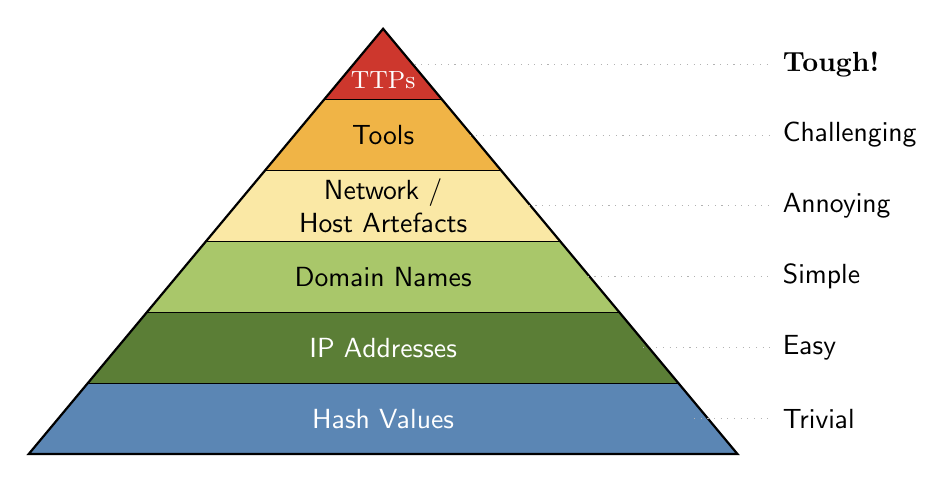
\begin{tikzpicture}[font=\sffamily, every node/.style={inner sep=2pt}]
    % Bianco's tiers --- colours approximated from the canonical diagram
    \definecolor{popTtps}{RGB}{205,55,45}
    \definecolor{popTools}{RGB}{240,180,70}
    \definecolor{popArt}{RGB}{250,232,165}
    \definecolor{popDom}{RGB}{169,199,106}
    \definecolor{popIp}{RGB}{91,126,54}
    \definecolor{popHash}{RGB}{91,134,180}

    % Geometry: half-base 4.5cm, height 5.4cm, six equal bands of 0.9cm.
    % Half-width at boundary y is 4.5*(1-y/5.4):
    %   y=0.0 -> 4.50    y=2.7 -> 2.25
    %   y=0.9 -> 3.75    y=3.6 -> 1.50
    %   y=1.8 -> 3.00    y=4.5 -> 0.75    y=5.4 -> 0.00 (apex)

    \fill[popHash]  (-4.50,0.0) -- (4.50,0.0) -- (3.75,0.9) -- (-3.75,0.9) -- cycle;
    \fill[popIp]    (-3.75,0.9) -- (3.75,0.9) -- (3.00,1.8) -- (-3.00,1.8) -- cycle;
    \fill[popDom]   (-3.00,1.8) -- (3.00,1.8) -- (2.25,2.7) -- (-2.25,2.7) -- cycle;
    \fill[popArt]   (-2.25,2.7) -- (2.25,2.7) -- (1.50,3.6) -- (-1.50,3.6) -- cycle;
    \fill[popTools] (-1.50,3.6) -- (1.50,3.6) -- (0.75,4.5) -- (-0.75,4.5) -- cycle;
    \fill[popTtps]  (-0.75,4.5) -- (0.75,4.5) -- (0.00,5.4) -- cycle;

    % Outline and tier separators
    \draw[black, thick] (-4.5,0) -- (4.5,0) -- (0,5.4) -- cycle;
    \draw[black]        (-3.75,0.9) -- (3.75,0.9);
    \draw[black]        (-3.00,1.8) -- (3.00,1.8);
    \draw[black]        (-2.25,2.7) -- (2.25,2.7);
    \draw[black]        (-1.50,3.6) -- (1.50,3.6);
    \draw[black]        (-0.75,4.5) -- (0.75,4.5);

    % Tier labels (inside each band; white text on dark fills)
    \node[text=white]                       at (0,0.45) {Hash Values};
    \node[text=white]                       at (0,1.35) {IP Addresses};
    \node                                   at (0,2.25) {Domain Names};
    \node[align=center]                     at (0,3.15) {Network /\\ Host Artefacts};
    \node                                   at (0,4.05) {Tools};
    \node[text=white, font=\small]          at (0,4.75) {TTPs};

    % Pain descriptors (right of pyramid)
    \node[anchor=west]                      at (5.0,0.45) {Trivial};
    \node[anchor=west]                      at (5.0,1.35) {Easy};
    \node[anchor=west]                      at (5.0,2.25) {Simple};
    \node[anchor=west]                      at (5.0,3.15) {Annoying};
    \node[anchor=west]                      at (5.0,4.05) {Challenging};
    \node[anchor=west, font=\bfseries]      at (5.0,4.95) {Tough!};

    % Dotted leaders from pyramid right edge to labels
    \draw[gray!60, dotted] (3.95,0.45) -- (4.95,0.45);
    \draw[gray!60, dotted] (3.30,1.35) -- (4.95,1.35);
    \draw[gray!60, dotted] (2.60,2.25) -- (4.95,2.25);
    \draw[gray!60, dotted] (1.85,3.15) -- (4.95,3.15);
    \draw[gray!60, dotted] (1.10,4.05) -- (4.95,4.05);
    \draw[gray!60, dotted] (0.40,4.95) -- (4.95,4.95);
  \end{tikzpicture}%
  }
  \caption{The Pyramid of Pain. Six tiers of indicators ordered by
  the cost imposed on an adversary when a defender denies that
  indicator class. Adapted from Bianco \cite{bianco2013}.}
  \label{fig:pop}
\end{figure}

The pyramid is a practitioner heuristic, not an empirically calibrated model, but the ordering it asserts is corroborated by peer-reviewed work on indicator durability. Sadlek et al.\ \cite{sadlek2022} identify TTPs as ``the most mature indicators used for the security defense''~\cite[p.~3]{sadlek2022}, placing them in a behavioural class categorically distinct from the disposable atomic indicators at the base: the validity of an IP address decays within a day~\cite{sadlek2022}, whereas behavioural patterns persist as long as the adversary's operational habits do. That durability is the point. Behaviour at the TTP rung is stable enough to model an adversary against, and it is the rung MTD claims to disrupt --- the asymmetry the rest of this review develops.



\subsection{Advanced Persistent Threats}
\label{subsec:apt}

Advanced Persistent Threat (APT) is a class of cyber threat in
which a well-resourced adversary --- typically nation-state or
organisation-sponsored --- pursues a specific objective against a
specific target over an extended time horizon, adapting to defender
resistance and retooling at a tempo that outpaces reactive defence
\cite{alshamrani2019}. The three terms name three properties:
\emph{advanced} tooling and tradecraft (custom malware, coordinated
attack vectors), a \emph{persistent} low-and-slow tempo that trades
speed for evasion across months or years, and a \emph{threat}
defined by its objective --- data exfiltration, impediment of
mission-critical components, or positioning for future
operations~\cite{alshamrani2019}. NIST states the same profile
behaviourally: an APT actor pursues its objectives repeatedly,
adapts to the defender's resistance, and sustains the interaction
needed to meet its goal \cite{alshamrani2019}. This is precisely
what the commodity attacker is not --- single-run, smash-and-grab
operations that neither hide nor adapt and end at first detection
\cite{alshamrani2019}.

APT operations follow a recognisable five-phase lifecycle:
reconnaissance, foothold establishment, lateral movement,
exfiltration or impediment, and post-operation cleanup
\cite{alshamrani2019}. The first two phases are invariant; the
remaining three are contingent on the adversary's objective ---
data theft, disruption of mission-critical components, or
positioning for future operations, the last of which may forgo
exfiltration entirely~\cite{alshamrani2019}.

APT campaigns are well-documented in the CTI record. The MITRE
ATT\&CK framework catalogues attributed operations, linking named
groups to their campaigns and software families at technique
resolution~\cite{alsada2024}, and examples such as
APT29 (Cozy Bear), Lazarus Group, and Volt Typhoon each carry dozens
of observed techniques across multiple operations. The Attack Flow
project \cite{ctid2025attackflow} curates these incidents into
structured records, and across them a group's toolchains and
sequencing recur from one operation to the next --- the consistency
analysts rely on for attribution. Because APT behaviour is both
well-documented and recurrent, it can be reconstructed into a
reusable adversarial profile rather than replayed as a single
incident. Unlike the heterogeneity of commodity attackers, this
makes the APT an appropriate adversary to model when evaluating
defences whose value scales with multi-step commitment. The next
subsection turns to attack profiling, the method that performs this
reconstruction.

\subsection{Attack Profiling}
\label{subsec:cti_profiling}

Attack profiling captures adversarial behaviour as structured representations: connecting individual tactics, techniques, and procedures into chains shaped by the attacker's objectives, motivations, and knowledge \cite{rodriguez2024}. CTI, the raw material for this work, ranges from low-level indicators of compromise to structured descriptions of TTPs, and in its unstructured form---narrative reports, blog posts, vendor write-ups---requires manual normalisation before systematic use \cite{ferraz2026}. The persistent obstacle is a procedural-semantic gap: CTI describes \emph{what} attackers do but routinely omits the sequencing, preconditions, and dependencies---the \emph{how}---required to operationalise behaviour as an executable or simulable process \cite{ferraz2026}.

Bridging this gap takes two forms --- manual curation and automated extraction --- that trade coverage against fidelity. The analyst-curated Attack Flow corpus (Section~\ref{subsec:mitre}) exemplifies the manual path: reliable structured representations from analyst review, at a pace and effort cost that limits coverage \cite{ctid2025attackflow}. Automated extraction dominates the literature~\cite{buchel2025} and spans three families: natural language processing (NLP), process mining (PM), and large language models (LLMs).

PM-based approaches, exemplified by Rodr{\'\i}guez et al.\ \cite{rodriguez2024}, discover attacker process models from labelled runtime event logs, recovering process structure in formalisms such as Petri nets; the manual cost shifts from narrative curation to authoring and maintaining the technique-labelling rules.

NLP-based approaches, exemplified by ChronoCTI \cite{rahman2025}, combine domain-fine-tuned language models with supervised classifiers to extract structured behaviour from text at scale: applied to 713 reports, it mines 124 recurring temporal patterns~\cite{rahman2025}, surfacing chains such as phishing followed by macro execution that individual reports describe in isolation.

LLM-based pipelines, exemplified by AttacKG+ \cite{zhangY2025}, replace the trained classifier with prompted LLM stages, the appeal being generalisation to unseen knowledge types without per-task training. However, a recent Systematization of Knowledge (SoK) on TTP extraction finds that generative and embedder-based methods do not yet beat traditional NLP classifiers in realistic open-set evaluation: even on the 50 most common TTPs, the best systems plateau near $F_1 = 0.70$ \cite{buchel2025}.

Of the two strands, automated extraction holds the coverage advantage, but on the SoK's evidence it does not yet recover technique-level behaviour reliably enough to ground an adversary on; manual curation supplies that fidelity, at the coverage cost noted above. Yet the whole apparatus for reconstructing behaviour from CTI --- automated and manual alike --- sits within the threat-intelligence and incident-response literature, the profiles this review motivates drawn from there rather than from the MTD evaluation Section~\ref{sec:convergence} turns to.

